\documentclass{article}

\usepackage[english]{babel}
\usepackage[square, numbers]{natbib}
\usepackage{url}
\bibliographystyle{abbrvnat}
\setcitestyle{authoryear,open={(},close={)}}

\usepackage[utf8]{inputenc}
\usepackage{amsmath}
\usepackage{amssymb}
\usepackage{amsthm}
\usepackage{physics}
\usepackage{gensymb}
\usepackage{verbatim}
\usepackage{amsfonts}
\usepackage{mathrsfs}
\usepackage{tikz-cd}
\usepackage{graphicx}
\usepackage{microtype}
\usepackage{centernot}
\usepackage{mathtools}
\usepackage[margin=1.0in]{geometry}
\usepackage{algorithm, algpseudocode}
\usepackage{bm}
\usepackage{caption}
\usepackage{enumitem}

\usepackage{pgfplots}
\pgfplotsset{compat=newest}
\usepackage{tikz}
\usetikzlibrary{shapes, positioning, quotes}


\usepackage[title]{appendix}
\usepackage{cleveref}
\usepackage{fancyhdr}
\usepackage{setspace}

\onehalfspacing

\pgfplotsset{height=8cm, width=15cm,compat=1.9}

\DeclareMathOperator*{\esssup}{ess\,sup}
\DeclareMathOperator*{\argmin}{arg\,min}
\DeclareMathOperator*{\argmax}{arg\,max}
\newcommand{\Ex}{\mathbb{E}}
\newcommand{\R}{\mathbb{R}}
\newcommand{\N}{\mathbb{N}}
\newcommand*\diff{\mathop{}\!\mathrm{d}}
\newcommand*\Diff[1]{\mathop{}\!\mathrm{d^#1}}
\newcommand{\w}{{\bf w}}
\newcommand{\bellman}{\mathcal{T}}
\newcommand{\statespace}{\mathcal{S}}
\newcommand{\actionspace}{\mathcal{A}}
\newcommand{\rewardfunction}{r}
\newcommand{\vpi}{V^\pi}
\newcommand{\qpi}{Q^\pi}
\newcommand{\qstar}{Q^*}
\newcommand{\vstar}{V^*}
\newcommand{\algname}{value inversion}
\newcommand{\Algname}{Value inversion}
\newcommand{\functionspace}{\mathcal{F}}
\newcommand{\KL}{\mathrm{KL}}
\newcommand{\policyparams}{\theta}
\newcommand{\boltzmannQ}{\mathcal{B}Q}
\newcommand{\entropy}{\mathrm{H}}
\newcommand{\piold}{{\pi_\mathrm{old}}}
\newcommand{\pinew}{{\pi_\mathrm{new}}}

\newtheorem{definition}{Definition}
\newtheorem{exercise}{Exercise}
\newtheorem{theorem}{Theorem}
\newtheorem{proposition}{Proposition}
\newtheorem{example}{Example}
\newtheorem{lemma}{Lemma}
\newtheorem{corollary}{Corollary}


% \pagestyle{fancy}
% \fancyhf{}
% \rhead{}
% \chead{Actor-Expert Notes}
% \lhead{}
% \rfoot{Page \thepage}
\title{KL Stuff}
\date{}

\begin{document}
\maketitle
\section{Theory}
\begin{enumerate}
    \item 
\end{enumerate}

\section{Experiments}


\subsection{Finite State, Finite Action Domains}
Sweeping over: softQtemp, softmaxtemp, actor learning rate, critic learning rate, epsilon
\begin{enumerate}
    \item FiveWorld (finite state, finite action): want to test short-term sacrifices for higher return
    \item Bandit (finite state, finite action): optimization landscape?
\end{enumerate}

\textbf{Questions}: In the case without function approximation (most ideal), which should we use? When we can control function approximation error (e.g., by perturbation) which should we use? How does each alg perform with respect to different policy initializations (e.g., initialize policy to take suboptimal path)?

\subsection{Finite State, Continuous Action}
Sweeping over: softQtemp, softmaxtemp, actor learning rate, critic learning rate, epsilon
\begin{enumerate}
    \item Continuous bandit
    \item ContinuousFiveWorld?
\end{enumerate}
\textbf{Questions}: 
Show mode-seeking and mean-seeking behavior.
W/o errors introduced by state function approximation, is doing forward KL feasible? (i.e., with numerical integration)


\subsection{Continuous State, Finite/Continuous Action}
Sweeping over: temperature, actor learning rate, critic learning rate
Technically there are two temperatures, but not feasible to sweep over both temperatures in deep. 
Will set softmax temperature to 1.
\begin{enumerate}
    \item Pendulum
    \item Mujoco env.
    %\item Possibly Minatar if there is time
\end{enumerate}

\textbf{Questions}: Is performance better?


\section{Rough Work}
\subsection{Necessity of Visitation Distribution Weighting}
Suppose $\eta(\pi_1) \geq \eta(\pi_2)$, where $\eta(\pi) := \Ex_\mu[v^\pi(s)]$ for some initial state distribution $\mu$. Using the classical performance difference lemma on $\eta(\pi_2)$ \citep{kakade2002approximately}, we have 
\begin{align*}
    \eta(\pi_2) &= \eta(\pi_1) + \frac{1}{1 - \gamma} \Ex_{\pi_2, d^{\pi_2}_\mu}[A^{\pi_1}(s, a)] \geq \eta(\pi_1)\\
    \Ex_{\pi_2, d^{\pi_2}_\mu}[A^{\pi_1}(s, a)] &\geq 0
\end{align*}
This leaves open the question of whether a different distribution would give a performance improvement on some subset of states, or the possibility of high-probability performance differences. 

% \subsection{Reparametrization Trick for Forward KL}
% The objective is 
% \begin{equation}
%     \KL(\boltzmannQ(s, \cdot) \parallel, \pi_\policyparams(\cdot \mid s)) = - \entropy(\boltzmannQ(s, \cdot)) - \int_\actionspace \boltzmannQ(s, a) \log \pi_\policyparams(a \mid s)\, da.
% \end{equation}
% %
% If we use reparametrization, we can write $a = f_\policyparams(s) + \epsilon$, where $\epsilon$ is drawn from some noise distribution. Hence,
% \begin{align*}
%     \nabla_\policyparams \KL(\boltzmannQ(s, \cdot) \parallel, \pi_\policyparams(\cdot \mid s)) &= -\int_\actionspace \nabla_\policyparams \boltzmannQ(s, a) \log \pi_\policyparams(a \mid s)\, da - \int_\actionspace  \boltzmannQ(s, a) \nabla_\policyparams \log \pi_\policyparams(a \mid s)\, da.\\
%     &= 
% \end{align*}


\subsection{Forward KL Counterexample}
Let us show that minimizing the forward KL between $\boltzmannQ$ and $\pi$ does not necessarily result in policy improvement, in contrast to minimizing the reverse KL. 

\begin{lemma}\label{lem:stronger-sac}
Let $\piold \in \Pi$ by some policy in our policy class $\Pi$. Let $\pinew$ be such that for each state $s$,
\begin{equation}
    \KL(\piold(\cdot \mid s) \parallel \boltzmannQ^\piold(s, \cdot)) \geq \KL(\pinew(\cdot \mid s) \parallel \boltzmannQ^\piold(s, \cdot)).
\end{equation}
Then for all $(s, a)$, we have $Q^\pinew(s, a) \geq Q^\piold(s, a)$, where $Q$ is a soft action-value.
\end{lemma}

\begin{lemma}\label{lem:forward-kl-counterexample}
There exists an MDP, a state $s'$, an initial policy $\piold$, and policy $\pinew$ such that the following are true for any temperature $\tau > 0$.
\begin{align}
    \forall s \in S,\, \KL(\boltzmannQ^\piold(s, \cdot) \parallel \piold(\cdot \mid s)) &\geq \KL(\boltzmannQ^\piold(s, \cdot) \parallel \pinew(\cdot \mid s)),\\
    \forall a \in \actionspace, \, Q^\pinew(s', a) &< Q^\piold(s', a).
\end{align}
Here again, $Q$ is a soft action-value of temperature $\tau$. 
% AC: actually, in the counterexample constructed \tau could be anything
\end{lemma}
\begin{proof}
Let us first construct the MDP. For simplicity, let us assume $\gamma = 1$ and we have an episodic MDP. 

\begin{center}
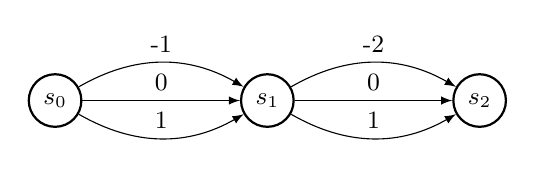
\begin{tikzpicture}[auto,node distance=10mm,>=latex,font=\small]
    \tikzstyle{round}=[thick,draw=black,circle]

    \node[round] (s0) {$s_0$};
    \node[round,right=20mm of s0] (s1) {$s_1$};
    \node[round,right=20mm of s1] (s2) {$s_2$};

    \draw[->] (s0) -- node {0} (s1);
    \draw [->] (s0) to [out=30,in=150] node {-1} (s1);
    \draw [->] (s0) to [out=-30,in=210] node {1} (s1);
    \draw[->] (s1) --  node{0}(s2);
    \draw [->] (s1) to [out=30,in=150] node{-2} (s2);
    \draw [->] (s1) to [out=-30,in=210] node {1} (s2);
    % \draw[->] (s0) [out=40,in=100,loop] to coordinate[pos=0.1](aa) (s0);
\end{tikzpicture}
\end{center}
%

$s_2$ is the terminal state and $s_0$ is the starting state. The numbers near the arrows represent the reward upon taking the action corresponding to an arrow, from a state. From top to bottom, we have action $a_0, a_1, a_2$. Let our initial policy $\piold$ be the equiprobable policy for all states and actions. That is, $\forall\, (s, a)$, $\piold(a \mid s) = \frac{1}{3}$. Consider $\pinew$ to be the following. 
\begin{align*}
    \pinew(\cdot \mid s_0) &= \piold(\cdot \mid s_0)\\
    \pinew(a_0 \mid s_1) &= 9/24\\
    \pinew(a_1 \mid s_1) &= 1 - 18/24\\
    \pinew(a_2 \mid s_1) &= 9/24
\end{align*}
%
By inspection, we have the soft value function of $\piold$ at $s_1$.
\begin{equation}
    V^\piold(s_1) = -1/3  + \ln 3    
\end{equation}
The soft action-value of $\piold$ is 
\begin{align*}
    Q^\piold(s_0, a_0) &= -1 + \tau^{-1} V^\piold(s_1)\\
    Q^\piold(s_0, a_1) &= 0 + \tau^{-1} V^\piold(s_1)\\
    Q^\piold(s_0, a_2) &= 1 + \tau^{-1} V^\piold(s_1)\\
    Q^\piold(s_1, a_0) &= -2\\
    Q^\piold(s_1, a_1) &= 0 \\
    Q^\piold(s_1, a_2) &= 1 \\
\end{align*}
The Boltzmann Q function follows, noting additionally that the softmax operator is invariant to constant shifts. 
\begin{align*}
    Z(s_0) &= \exp(\tau^{-1} V^\piold(s_1))(1 + \exp(1) + \exp(-1)) \\
    Z(s_1) &= 1 + \exp(1) + \exp{-2}\\
    \boltzmannQ^\piold(s_0, a_0) &= \frac{\exp(-1)}{Z(s_1)}\\
    \boltzmannQ^\piold(s_0, a_1) &= \frac{1}{Z(s_1)}\\
    \boltzmannQ^\piold(s_0, a_2) &= \frac{\exp(1)}{Z(s_1)}\\
    \boltzmannQ^\piold(s_1, a_0) &= \frac{\exp(-2)}{Z(s_1)}\\
    \boltzmannQ^\piold(s_1, a_1) &= \frac{1}{Z(s_1)}\\
    \boltzmannQ^\piold(s_1, a_2) &= \frac{\exp(1)}{Z(s_1)}
\end{align*}
The new soft action value at $s_0$ is given by the following.  
\begin{align*}
    Q^\pinew(s_0, a_0) &= -1 - \frac{3}{8} + \tau^{-1}\entropy(\pinew(\cdot \mid s_1))\\
    Q^\pinew(s_0, a_1) &= 0 - \frac{3}{8} + \tau^{-1}\entropy(\pinew(\cdot \mid s_1))\\
    Q^\pinew(s_0, a_2) &= 1 - \frac{3}{8} + \tau^{-1}\entropy(\pinew(\cdot \mid s_1))
\end{align*}
Since entropy is maximized by a uniform distribution and since $-3/8 < -3/9 = -1/3$, we clearly have that $Q^\pinew(s_0, a) < Q^\piold(s_0, a)$ for all actions $a$. Calculating the forward KL divergences,
\begin{align*}
    % \KL(\boltzmannQ^\piold(s_0, \cdot) \parallel \piold(\cdot \mid s_0)) &= -\entropy(\boltzmannQ^\piold(s_0, \cdot)) - \frac{1}{Z(s_1)} (\exp(-1) \log(1/3) + \log(1/3) + \exp(1) \log(1/3))  \\
    \KL(\boltzmannQ^\piold(s_0, \cdot) \parallel \pinew(\cdot \mid s_0)) &= \KL(\boltzmannQ^\piold(s_0, \cdot) \parallel \piold(\cdot \mid s_0)) \\
    \KL(\boltzmannQ^\piold(s_1, \cdot) \parallel \piold(\cdot \mid s_1)) &= -\entropy(\boltzmannQ^\piold(s_1, \cdot)) - \frac{1}{Z(s_1)}  (\exp(-2) \log(1/3) + \log(1/3) + \exp(1) \log(1/3)) \\
    \KL(\boltzmannQ^\piold(s_1, \cdot) \parallel \pinew(\cdot \mid s_1)) &= -\entropy(\boltzmannQ^\piold(s_1, \cdot)) - \frac{1}{Z(s_1)}  (\exp(-2) \log(9/24) + \log(6/24) + \exp(1) \log(9/24)) 
\end{align*}
It suffices to ignore $-\entropy(\boltzmannQ^\piold(s_1, \cdot))$. We have 
\begin{align*}
    (\exp(-2) \log(1/3) + \log(1/3) + \exp(1) \log(1/3)) &\approx -1.83864\\
    (\exp(-2) \log(9/24) + \log(6/24) + \exp(1) \log(9/24)) &\approx -1.81761
\end{align*}
Hence, 
\begin{equation}
      \KL(\boltzmannQ^\piold(s_1, \cdot) \parallel \piold(\cdot \mid s_1)) > \KL(\boltzmannQ^\piold(s_1, \cdot) \parallel \pinew(\cdot \mid s_1))
\end{equation}
\end{proof}

\subsection{Minimization of the Reverse KL on Average Gives Policy Improvement}
Our goal here is to understand if we can attain policy improvement by ensuring that our new policy is lower in reverse KL than the old policy \textit{on average} across states, rather than across all states. This case is important in the function-approximation regime, when we usually \textit{cannot} ensure an improvement in reverse KL for every state. 


The following ``soft'' counterpart to the performance difference lemma \citep{kakade2002approximately,schulman2015trust} will be useful. 
\begin{lemma}[Soft Performance Difference]\label{lemma:soft-performance-difference}
Let $\pi_1$, $\pi_2$ be policies and let $Q_1$, $V_1$, and $A_1$ respectively be the soft action value, soft state value, and $Q_1 - V_1$. Let $\rho^{\pi_2}$ be the future state visitation distribution of $\pi_2$. Let $\eta(\pi) := \Ex_{s_0}[V^\pi(s)]$ be the average soft performance of $\pi$. Then 
\begin{equation}
    \frac{1}{1 - \gamma}\Ex_{\rho^{\pi_2}}[A_1(s, a)] + \eta(\pi_1) = \eta(\pi_2) - \frac{1}{1- \gamma} \Ex_{\rho^{\pi_2}}[\entropy(\pi_2(\cdot \mid s))]
\end{equation}
\end{lemma}
\begin{proof}
Fix some distribution of starting states. Below, we will write $\Ex_{p, \pi}$ to denote the expectation when drawing trajectories generated according to $p$ and $\pi_2$, with starting state distribution fixed. We calculate as in \citet{kakade2002approximately,schulman2015trust}.
\begin{align*}
    \frac{1}{1 - \gamma} \Ex_{\rho^{\pi_2}}[A_1(s, a)] &= \Ex_{p, \pi_2}\left[\sum_{t = 0}^\infty \gamma^t A_1(s_t, a_t)\right]\\
        &= \Ex_{p, \pi_2}\left[\sum_{t = 0}^\infty \gamma^t (r(s_t, a_t) + \gamma V_1(s_{t + 1}) - V_1(s_t))\right]\\
        &= \Ex_{p, \pi_2}\left[\sum_{t = 0}^\infty \gamma^t r(s_t, a_t) - V_1(s_0)\right]\\
        &= -\eta(\pi_1) + \Ex_{p, \pi_2}\left[\sum_{t = 0}^\infty \gamma^t r(s_t, a_t) \right]\\
        &= -\eta(\pi_1) + \Ex_{p, \pi_2}\left[\sum_{t = 0}^\infty \gamma^t (r(s_t, a_t) - \log \pi_2(a_t \mid s_t)) \right] + \Ex_{p, \pi_2}\left[\sum_{t = 0}^\infty \gamma^t\log \pi_2(a_t \mid s_t) \right]\\
        &= -\eta(\pi_1) + \eta(\pi_2)  - \frac{1}{1 - \gamma} \Ex_{\rho^{\pi_2}}[\entropy(\pi_2(\cdot \mid s))]
\end{align*}
\end{proof}

We thus have the following proposition. 
\begin{proposition}\label{prop:avg-reverse-kl}
Fix a policy class $\Pi$ and let $\pi_1 \in \Pi$. Let $Q_1, V_1$ be the corresponding action-value and state value functions for $\pi_1$. Let $\pi_2 \in \Pi$ be a policy such that
\begin{equation}
    \Ex_{\rho^{\pi_2}}[\KL(\pi_1(\cdot \mid s) \parallel \boltzmannQ_1(s, \cdot))] \geq \Ex_{\rho^{\pi_2}}[\KL(\pi_2(\cdot \mid s) \parallel \boltzmannQ_1(s, \cdot))].
\end{equation}
Fix some distribution over starting states $\mu$. Let $\eta(\pi) := \Ex_\mu[V^\pi(s_0)]$ (note that $V^\pi$ might be a soft value function). Assume furthermore that $\Ex_{\rho^{\pi_2}}[\entropy(\pi_1(\cdot \mid s) - \entropy(\pi_2(\cdot \mid s))] \geq 0$. Then the following holds. 
\begin{equation}
    \eta(\pi_2) \geq \eta(\pi_1)
\end{equation}
\end{proposition}
\begin{proof}
We calculate. 
\begin{align*}
    \Ex_{\rho^{\pi_2}}[\KL(\pi_1(\cdot \mid s) \parallel \boltzmannQ_1(s, \cdot))] &\geq \Ex_{\rho^{\pi_2}}[\KL(\pi_2(\cdot \mid s) \parallel \boltzmannQ_1(s, \cdot))]\\
    \Ex_{\rho^{\pi_2}}[\Ex_{\pi_1}[\log \pi_1(\cdot \mid s)] - V_1(s)] &\geq \Ex_{\rho^{\pi_2}}[\Ex_{\pi_2}[\log \pi_2(\cdot \mid s) - Q_1(s, \cdot)]\\
    \Ex_{\rho^{\pi_2}}[\Ex_{\pi_2}[Q_1(s, a) - V_1(s)]] &\geq \Ex_{\rho^{\pi_2}}[\entropy(\pi_1(\cdot \mid s) - \entropy(\pi_2(\cdot \mid s))]
\end{align*}
Assume that our value functions are not soft. By the performance difference lemma \citep{kakade2002approximately,schulman2015trust}, we have that $\pi_2$ is better than $\pi_1$ if $\Ex_{\rho^{\pi_2}}[\entropy(\pi_1(\cdot \mid s) - \entropy(\pi_2(\cdot \mid s))] \geq 0$. Intuitively, $\pi_2$ must ``commit'' more than $\pi_1$ on average. 

Now assume that our value functions are soft. Using \Cref{lemma:soft-performance-difference}, we have that $\Ex_{\rho^{\pi_2}}[\entropy(\pi_1(\cdot \mid s) - \entropy(\pi_2(\cdot \mid s))] \geq 0$ implies
\begin{equation}
    \eta(\pi_1) \leq \eta(\pi_2) - \frac{1}{1- \gamma} \Ex_{\rho^{\pi_2}}[\entropy(\pi_2(\cdot \mid s))] \leq \eta(\pi_2).
\end{equation}

\end{proof}

\subsection{Linear FA with Forward KL}
Our goal here is to show that optimizing the forward KL can give us a policy $\pi_2$ that satisfies the conditions of \Cref{prop:avg-reverse-kl}. If we use linear function approximation for the policy over a softmax, then the forward KL is convex with respect to $\policyparams$. 

\begin{proposition}
Let $\phi(s, a)$ be a feature vector for every $(s, a) \in \statespace \times \actionspace$. Fix some distribution $\mu$ over states. Assume that for all $(s, a) \in \statespace \times \actionspace$, $\pi_\policyparams(a \mid s) \propto \exp(\policyparams^\top \phi(s, a))$. Fix some initial parameters $\policyparams_1$ and let $Q_1 := Q^{\pi_{\policyparams_1}}$. Define the state-value function and the advantage function of $\pi_{\policyparams_1}$ analagously. These value functions may be either soft or not soft. Let $\policyparams_2$ be such that 
\begin{equation}
    \policyparams_2 \in \argmin_{\policyparams} \Ex_\mu\left[\KL(\boltzmannQ_1(s, \cdot) \parallel \pi_\policyparams(\cdot \mid s))\right],
\end{equation}
which we assume to exist.
Assume as well that
\begin{equation}\label{eq:strong-assumption}
    - \Ex_\mu\left[\left(\nabla_\policyparams \KL(\boltzmannQ_1(s, \cdot) \parallel \pi_{\policyparams_1}(\cdot \mid s)\right)\right]^\top \policyparams_2 &\leq \Ex_\mu\left[\sum_a A_1(s, a) \pi_{\policyparams_2}(a \mid s)\right].
\end{equation}
Then
\begin{equation}
    \Ex_\mu[\KL( \pi_{\policyparams_2}(\cdot \mid s) \parallel \boltzmannQ_1(s, \cdot))] \leq \Ex_\mu[\KL( \pi_{\policyparams_1}(\cdot \mid s) \parallel \boltzmannQ_1(s, \cdot))]
\end{equation}
\end{proposition}
\begin{proof}
% still true with expectation?
To avoid notational clutter, we will work with a single state $s$. The general result follows since everything we do will be true under expectation, given linearity and monotonicity of expectations. 

Let us first try to derive some properties of $\policyparams_2$. We have the following expression for the entropy of a linear softmax policy. 
\begin{align*}
    \entropy(\pi_{\policyparams}(\cdot \mid s)) &= -\sum_a \pi_{\policyparams} (a \mid s) \log \pi_{\policyparams} (a \mid s) \\
    &=  -\sum_a \pi_{\policyparams} (a \mid s) \left(\policyparams^\top \phi(s, a) - \log\left( \sum_b \exp(\policyparams^\top \phi(s, b)) \right)\right)\\
    &= -\sum_a \pi_{\policyparams} (a \mid s)\policyparams^\top \phi(s, a) + \log\left( \sum_b \exp(\policyparams^\top \phi(s, b)) \right)
\end{align*}

The forward KL and its gradient are given by
\begin{align*}
    \KL(\boltzmannQ_1(s, \cdot) \parallel \pi_\policyparams(\cdot \mid s)) &= -\entropy(\boltzmannQ_1(s, \cdot)) - \sum_a \boltzmannQ_1(s, a) \log \pi_\policyparams(a \mid s)\\
        &= -\entropy(\boltzmannQ_1(s, \cdot)) - \sum_a \boltzmannQ_1(s, a)\left(\policyparams^\top \phi(s, a) - \log\left( \sum_b \exp(\policyparams^\top \phi(s, b)) \right)\right)\\
        &= -\entropy(\boltzmannQ_1(s, \cdot)) - \sum_a \boltzmannQ_1(s, a) \policyparams^\top \phi(s, a) + \log\left( \sum_b \exp(\policyparams^\top \phi(s, b)) \right)\\
    \nabla_\theta \KL(\boltzmannQ_1(s, \cdot) \parallel \pi_\policyparams(\cdot \mid s)) &=  - \sum_a \boltzmannQ_1(s, a) \phi(s, a) + \sum_b \phi(s, b) \pi_\policyparams(b \mid s)
\end{align*}

Setting the gradient to be zero, a global minimum $\policyparams_2$ must satisfy the following.
\begin{align*}
    \sum_a \boltzmannQ_1(s, a) \phi(s, a) &= \sum_b \phi(s, b) \pi_{\policyparams_2}(b \mid s).
\end{align*}
Hence, 
\begin{align*}
    \KL(\boltzmannQ_1(s, \cdot) \parallel \pi_{\policyparams_2}(\cdot \mid s)) &= -\entropy(\boltzmannQ_1(s, \cdot)) - \sum_a \pi_{\policyparams_2}(a \mid s) \policyparams^\top \phi(s, a) + \log\left( \sum_b \exp(\policyparams_2^\top \phi(s, b)) \right)\\
    &= \entropy(\pi_{\policyparams_2}(\cdot \mid s)) - \entropy(\boltzmannQ_1(s, \cdot))
\end{align*}
Additionally, for any other $\policyparams$, we have by convexity of the forward KL and the first-order convexity condition that 
\begin{align*}
    \KL(\boltzmannQ_1(s, \cdot) \parallel \pi_{\policyparams_2}(\cdot \mid s)) -  \KL(\boltzmannQ_1(s, \cdot) \parallel \pi_{\policyparams_1}(\cdot \mid s)) &\geq \left(\nabla_\policyparams \KL(\boltzmannQ_1(s, \cdot) \parallel \pi_{\policyparams_1}(\cdot \mid s)\right)^\top (\policyparams_2 - \policyparams_1)\\
\end{align*}
By using the expression for the forward KL of $\policyparams_2$ and expanding the forward KL of $\policyparams_1$, the left-hand side can be written as
\begin{equation*}
    \entropy(\pi_{\policyparams_2}(\cdot \mid s)) + \sum_a \boltzmannQ_1(s, a) \policyparams_1^\top \phi(s, a) - \log\left( \sum_b \exp(\policyparams_1^\top \phi(s,b)) \right)
\end{equation*}
By adding $\left(\nabla_\policyparams \KL(\boltzmannQ_1(s, \cdot) \parallel \pi_{\policyparams_1}(\cdot \mid s)\right)^\top \policyparams_1$ to both sides of the inequality, and simplifying, we obtain
\begin{align}
    %  \KL(\boltzmannQ_1(s, \cdot) \parallel \pi_{\policyparams_2}(\cdot \mid s)) -  \KL(\boltzmannQ_1(s, \cdot) \parallel \pi_{\policyparams_1}(\cdot \mid s)) &\geq \left(-\sum_a \boltzmannQ_1(s, a) \phi(s, a) + \sum_b \phi(s, b) \pi_\policyparams(b \mid s)\right)^\top (\policyparams_2 - \policyparams_1) \\
    %  \entropy(\pi_{\policyparams_2}(\cdot \mid s)) + \sum_a \boltzmannQ_1(s, a) \policyparams_1^\top \phi(s, a) - \log\left( \sum_b \exp(\policyparams_1^\top \phi(s, b)) \right) &\geq \left(-\sum_a \boltzmannQ_1(s, a) \phi(s, a) + \sum_b \phi(s, b) \pi_\policyparams(b \mid s)\right)^\top (\policyparams_2 - \policyparams_1)\\ 
     \entropy(\pi_{\policyparams_2}(\cdot \mid s)) - \log\left( \sum_b \exp(\policyparams_1^\top \phi(s, b)) \right) + \sum_b \policyparams_1^\top \phi(s, a) \pi_{\policyparams_1}(a \mid s) &\geq \left(\nabla_\policyparams \KL(\boltzmannQ_1(s, \cdot) \parallel \pi_{\policyparams_1}(\cdot \mid s)\right)^\top \policyparams_2\nonumber \\ 
     \entropy(\pi_{\policyparams_2}(\cdot \mid s)) - \entropy(\pi_{\policyparams_1}(\cdot \mid s)) &\geq \left(\nabla_\policyparams \KL(\boltzmannQ_1(s, \cdot) \parallel \pi_{\policyparams_1}(\cdot \mid s)\right)^\top \policyparams_2 \label{eq:first-order-convexity}
\end{align}
% As well, optimality of $\policyparams_2$ yields the following. 
% \begin{align*}
%     \KL(\boltzmannQ_1(s, \cdot) \parallel \pi_{\policyparams_2}(\cdot \mid s)) &\leq \KL(\boltzmannQ_1(s, \cdot) \parallel \pi_{\policyparams_1}(\cdot \mid s))\\
%     \entropy(\pi_{\policyparams_2}(\cdot \mid s)) &\leq - \sum_a \boltzmannQ_1(s, a) \policyparams_1^\top \phi(s, a) + \log\left( \sum_b \exp(\policyparams_1^\top \phi(s, b)) \right)
% \end{align*}
Let us now turn to the reverse KL. 
\begin{align*}
    \KL&( \pi_{\policyparams_2}(\cdot \mid s) \parallel \boltzmannQ_1(s, \cdot)) - \log Z(s) \\
    &= -\entropy(\pi_{\policyparams_2}(\cdot \mid s)) - \sum_a Q_1(s, a) \pi_{\policyparams_2}(a \mid s) \\
    &\leq - \entropy(\pi_{\policyparams_1}(\cdot \mid s)) - \sum_a Q_1(s, a) \pi_{\policyparams_2}(a \mid s)  - \left(\nabla_\policyparams \KL(\boltzmannQ_1(s, \cdot) \parallel \pi_{\policyparams_1}(\cdot \mid s)\right)^\top \policyparams_2\\
    &\leq -\entropy(\pi_{\policyparams_1}(\cdot \mid s)) - \sum_a Q_1(s, a) \pi_{\policyparams_1} (s, a)\\
    &= \KL( \pi_{\policyparams_1}(\cdot \mid s) \parallel \boltzmannQ_1(s, \cdot)) - \log Z(s)
\end{align*}
The third line is from \Cref{eq:first-order-convexity} and the fourth line is from \Cref{eq:strong-assumption}. 
\end{proof}
% To complete the proof, we want to show that 
% \begin{equation*}
%     - \sum_a Q_1(s, a) \pi_{\policyparams_2}(a \mid s) - \left(\nabla_\policyparams \KL(\boltzmannQ_1(s, \cdot) \parallel \pi_{\policyparams_1}(\cdot \mid s)\right)^\top \policyparams_2 \leq -\sum_a Q_1(s, a) \pi_{\policyparams_1}(a \mid s)
% \end{equation*}
% Equivalently, 
% \begin{align*}
%      \sum_a Q_1(s, a) \pi_{\policyparams_1}(a \mid s) - \left(\nabla_\policyparams \KL(\boltzmannQ_1(s, \cdot) \parallel \pi_{\policyparams_1}(\cdot \mid s)\right)^\top \policyparams_2 &\leq \sum_a Q_1(s, a) \pi_{\policyparams_2}(a \mid s)\\
%      V_1(s) - \left(\nabla_\policyparams \KL(\boltzmannQ_1(s, \cdot) \parallel \pi_{\policyparams_1}(\cdot \mid s)\right)^\top \policyparams_2 &\leq \sum_a A_1(s, a) \pi_{\policyparams_2}(a \mid s) + V_1(s)\\
%     - \left(\nabla_\policyparams \KL(\boltzmannQ_1(s, \cdot) \parallel \pi_{\policyparams_1}(\cdot \mid s)\right)^\top \policyparams_2 &\leq \sum_a A_1(s, a) \pi_{\policyparams_2}(a \mid s)\\
%     %  \sum_a Q_1(s, a) \pi_{\policyparams_1}(a \mid s) - \sum_a Q_1(s, a) \pi_{\policyparams_2}(a \mid s)\leq \left(\nabla_\policyparams \KL(\boltzmannQ_1(s, \cdot) \parallel \pi_{\policyparams_1}(\cdot \mid s)\right)^\top \policyparams_2
% \end{align*}
% We have 
% \begin{align*}
%     - \sum_a Q_1(s, a)& \pi_{\policyparams_2}(a \mid s) + \sum_a \boltzmannQ_1(s, a) \policyparams_2^\top \phi(s, a) - \sum_b \policyparams_2^\top \phi(s, b) \pi_{\policyparams_1}(b \mid s)\\
%     &\leq \log\left( \sum_a \exp(\policyparams_1^\top \phi(s, a)) \right) - \entropy(\pi_{\policyparams_2}(\cdot \mid s)) - \sum_a Q_1(s, a) \pi_{\policyparams_2}(a \mid s) - \sum_a \policyparams_2^\top \phi(s, a) \pi_{\policyparams_1}(a \mid s) \\
% \end{align*}
% If we assume that $\exists \, w_1$ such that $Q_1(s, a) = w_1^\top \phi(s, a)$, then 
% \begin{align*}
%     - \sum_a Q_1(s, a) &\pi_{\policyparams_2}(a \mid s) + \sum_a \pi_{\policyparams_2}(s, a) \policyparams_2^\top \phi(s, a) - \sum_b \policyparams_2^\top \phi(s, b) \pi_{\policyparams_1}(b \mid s) \\
%     &= \sum_a \phi(s, a)^\top (\pi_{\policyparams_2}(a \mid s) \policyparams_2 - \pi_{\policyparams_1}(a \mid s) \policyparams_2 - \pi_{\policyparams_2}(a \mid s) w_1)
% \end{align*}
% \subsection{Forward KL as a Surrogate for Reverse KL}
% Even though we might not have monotonic policy improvement with forward KL, it might still be a useful surrogate loss function for the reverse KL, especially since forward KL is convex with respect to the features of a softmax policy, while reverse KL is not. We want to be able to achieve a low reverse-KL loss on average by using the forward KL as a surrogate objective. We will follow the discussion in \citet{steinwart2007compare}. 

% First, fix some state $s \in S$ and policy $\piold$. 
% \begin{proposition}
% Let $s \in \statespace$. The forward KL is reverse-KL-calibrated. Additionally, fixing some distribution over states $\mu(s)$, for any $\epsilon > 0$ there is $\delta > 0$ such that 
% \begin{equation}
%     \Ex_\mu[L_2(s)] < \delta \implies \Ex_\mu[L_1(s)] < \epsilon
% \end{equation}
% \end{proposition}

\bibliography{refs}
\end{document}


% 